\documentclass{standalone}
\usepackage{fontspec}
\usepackage{sourcecodepro}
\usepackage{tikz}

\setmainfont{TeX Gyre Heros}
\setmonofont{Source Code Pro}

\usetikzlibrary{matrix, positioning, decorations.pathreplacing, calligraphy}

\tikzset{
  layout/.style={
    matrix of nodes,
    thick,
    row sep=-\pgflinewidth,
    %column sep=-\pgflinewidth,
    column sep=2pt,
    nodes={rectangle, draw=black, align=center, font=\ttfamily},
    minimum height=1.5em,
    text depth=0.5ex,
    text height=2ex,
    nodes in empty cells,
  },
  descr/.style={
    matrix of nodes,
    row sep=-\pgflinewidth,
    column sep=-\pgflinewidth,
    nodes={rectangle, align=right, draw=black},
    minimum height=1.5em,
    text depth=0.5ex,
    text height=2ex,
    nodes in empty cells,
    column 1/.style={anchor=base east},
  },
  header/.style={
    text width=10em
  },
  sizet/.style={
    text width=6.5em
  },
  arr/.style={
    text width=10em
  },
  legend/.style={
    decorate, decoration={calligraphic brace, amplitude=10pt, mirror}, line width=0.5pt,
    % node options
    align=center, midway, below
  }
}

\begin{document}
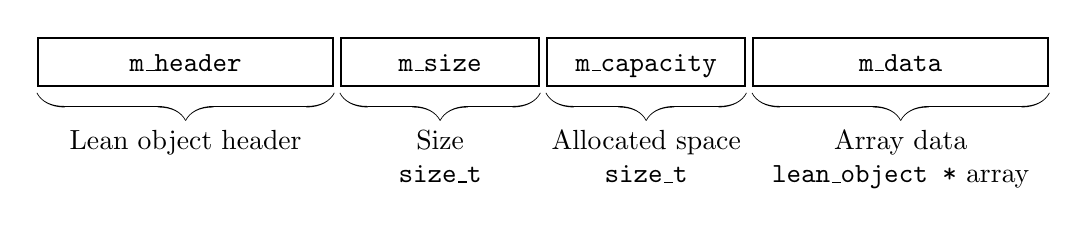
\begin{tikzpicture}
  \matrix (array) [layout] {
    \node[header](array-1-1){m\_header}; & \node[sizet](array-1-2){m\_size}; & \node[sizet](array-1-3){m\_capacity}; & \node[arr](array-1-4){m\_data}; \\
  };
  \draw[legend] ([yshift=-2pt] array-1-1.south west) -- ([yshift=-2pt]array-1-1.south east) node [midway, below, yshift=-1em] {Lean object header};
  \draw[legend] ([yshift=-2pt]array-1-2.south west) -- ([yshift=-2pt]array-1-2.south east) node [align=center,midway, below, yshift=-1em] {Size\\\texttt{size\_t}};
  \draw[legend] ([yshift=-2pt]array-1-3.south west) -- ([yshift=-2pt]array-1-3.south east) node [midway, below, yshift=-1em] {Allocated space\\\texttt{size\_t}};
  \draw[legend] ([yshift=-2pt]array-1-4.south west) -- ([yshift=-2pt]array-1-4.south east) node [midway, below, yshift=-1em] {Array data\\\texttt{lean\_object *} array};
\end{tikzpicture}
\end{document}

% Local Variables:
% TeX-engine: luatex
% End:
